\subsection{Anzahl Hinweise pro Band}

\begin{figure}[H]
    \centering
    \begin{minipage}{0.48\textwidth}
        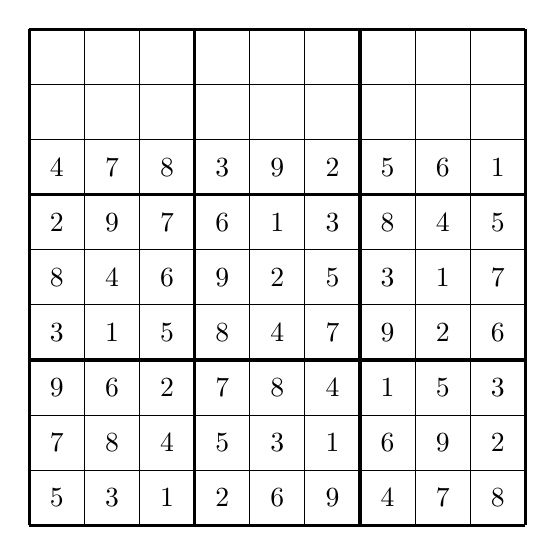
\begin{tikzpicture}
            % Zellgröße
            \def\s{0.7cm}

            % Sudoku-Lösung (kann beliebig angepasst werden)
            \def\sudoku{
                    {, , , , , , , , },
                    {, , , , , , , , },
                    {4, 7, 8, 3, 9, 2, 5, 6, 1},
                    {2, 9, 7, 6, 1, 3, 8, 4, 5},
                    {8, 4, 6, 9, 2, 5, 3, 1, 7},
                    {3, 1, 5, 8, 4, 7, 9, 2, 6},
                    {9, 6, 2, 7, 8, 4, 1, 5, 3},
                    {7, 8, 4, 5, 3, 1, 6, 9, 2},
                    {5, 3, 1, 2, 6, 9, 4, 7, 8},
            }

            % Rasterlinien
            \foreach \x in {0,1,...,9} {
                \draw[thin] (\x*\s, 0) -- (\x*\s, 9*\s);
                \draw[thin] (0, \x*\s) -- (9*\s, \x*\s);
            }
            \foreach \x in {0,3,6,9} {
                \draw[very thick] (\x*\s, 0) -- (\x*\s, 9*\s);
                \draw[very thick] (0, \x*\s) -- (9*\s, \x*\s);
            }




            % Zahlen eintragen
            \foreach \row [count=\i from 0] in \sudoku {
                \foreach \num [count=\j from 0] in \row {
                % Y-Koordinate: Startet oben bei 8.5 und geht pro Zeile 1 runter
                    \node at (\j*\s + 0.5*\s, 8.5*\s - \i*\s) {\num};
                }
            }
        \end{tikzpicture}
    \end{minipage}
    \hfill
    \begin{minipage}{0.48\textwidth}
        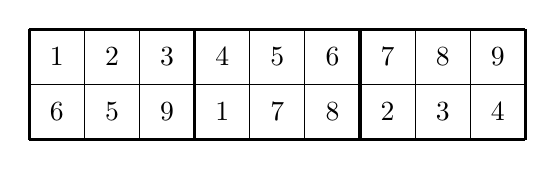
\begin{tikzpicture}[baseline]
            % Zellgröße
            \def\s{0.7cm}

            % Werte für das 2x9 Gitter
            \def\zweizeilen{
                    {1, 2, 3, 4, 5, 6, 7, 8, 9},
                    {6, 5, 9, 1, 7, 8, 2, 3, 4},
            }

            % Rasterlinien
            \foreach \x in {0,1,...,9} {
                \draw[thin] (\x*\s, 0) -- (\x*\s, 2*\s);
            }
            \foreach \y in {0,1,2} {
                \draw[thin] (0, \y*\s) -- (9*\s, \y*\s);
            }

            % Dickere Linien wie bei Sudoku
            \foreach \x in {0,3,6,9} {
                \draw[very thick] (\x*\s, 0) -- (\x*\s, 2*\s);
            }
            \draw[very thick] (0, 0) -- (9*\s, 0);
            \draw[very thick] (0, 2*\s) -- (9*\s, 2*\s);

            % Zahlen eintragen
            \foreach \row [count=\i from 0] in \zweizeilen {
                \foreach \num [count=\j from 0] in \row {
                    \node at (\j*\s + 0.5*\s, 1.5*\s - \i*\s) {\num};
                }
            }
        \end{tikzpicture}
        \\
        \\

        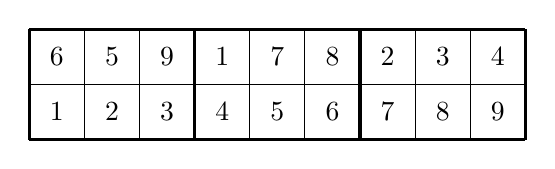
\begin{tikzpicture}[baseline]
            % Zellgröße
            \def\s{0.7cm}

            % Werte für das 2x9 Gitter
            \def\zweizeilen{
                    {6, 5, 9, 1, 7, 8, 2, 3, 4},
                    {1, 2, 3, 4, 5, 6, 7, 8, 9},
            }

            % Rasterlinien
            \foreach \x in {0,1,...,9} {
                \draw[thin] (\x*\s, 0) -- (\x*\s, 2*\s);
            }
            \foreach \y in {0,1,2} {
                \draw[thin] (0, \y*\s) -- (9*\s, \y*\s);
            }

            % Dickere Linien wie bei Sudoku
            \foreach \x in {0,3,6,9} {
                \draw[very thick] (\x*\s, 0) -- (\x*\s, 2*\s);
            }
            \draw[very thick] (0, 0) -- (9*\s, 0);
            \draw[very thick] (0, 2*\s) -- (9*\s, 2*\s);

            % Zahlen eintragen
            \foreach \row [count=\i from 0] in \zweizeilen {
                \foreach \num [count=\j from 0] in \row {
                    \node at (\j*\s + 0.5*\s, 1.5*\s - \i*\s) {\num};
                }
            }
        \end{tikzpicture}
    \end{minipage}
    \caption{Beispiel für Zeilenvertauschung}
    \label{fig:row_constraints}
\end{figure}

In einem partiellen Sudoku darf es in einem horizontalen Band keine zwei Zeilen ohne Hinweise geben.
In \cref{fig:row_constraints} kann man sehen das es ansonsten mehrere Lösungen gibt.
Alle Hinweise bis auf zwei komplette Zeilen sind gegeben und es gibt trotzdem zwei Lösungen, welche man rechts sehen kann.
Äquivalent dazu dürfen in einem vertikalen Band keine zwei Spalten ohne Hinweise sein.
Übersetzt man dies auf allgemeine Sudoku-Größen,
muss in einem Band der Breite beziehungsweise Höhe $n$ mindestens $n-1$ Spalten beziehungsweise Zeilen mit Hinweisen gegeben sein.
